\section{Auswertung}
\subsection{Ersatzschaltbild Transformator}
\begin{enumerate}[label=\alph*)]
	\item Zeichnen Sie das vollständige einphasige Ersatzschaltbild (Sternschaltung) des
	      Transformators.
	      \begin{figure}[h!]
		      \begin{center}
			      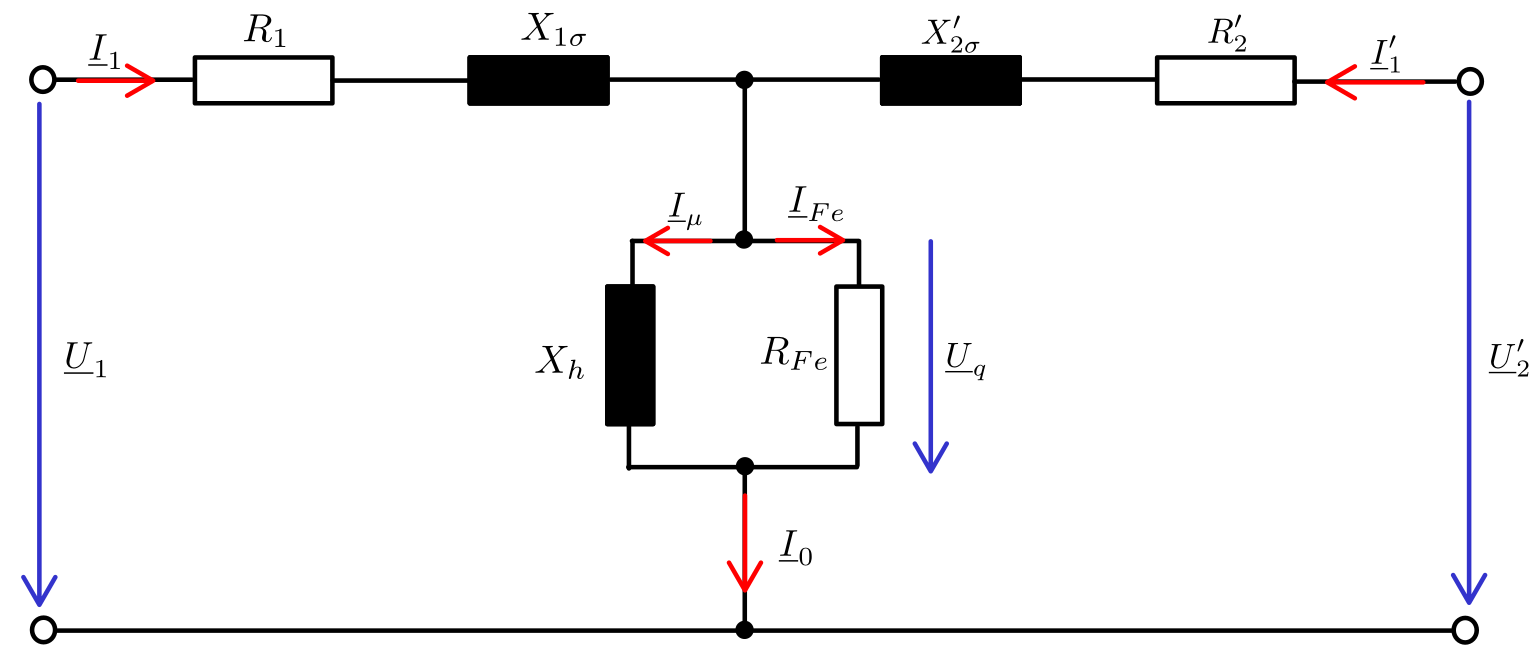
\includegraphics[width=0.95\textwidth]{img/4.1.1.1}
		      \end{center}
		      \caption{}\label{img:4.1.1.1}
	      \end{figure}

	\item Bestimmen Sie die Leistung im Leerlauf auf der Primärseite nach Gleichung (16).
	      \begin{align*}
		      \underline S & = \underline U_{12} \cdot \underline I_1^* + \underline U_{32}\cdot \underline I_3^* \\
		      \underline S & = \underline U_{12} \cdot \underline I_1^* - \underline U_{23}\cdot \underline I_3^* \\
		      \underline S & = 395\ V \cdot e^{j0^\circ} \cdot 0.45\ A \cdot e^{-(-j120^\circ)} -
		      393\ V \cdot e^{-j120^\circ}\cdot 0.45\ A \cdot e^{-(j45^\circ)}                                    \\
		      \underline S & = 81,9\ W + j199,7\ var = 327,6\ VA\cdot e^{j97,6^\circ}
	      \end{align*}

	\item Bestimmen Sie die Wirkleistung im Kurzschlussfall auf der Sekundärseite nach
	      Gleichung (16). Gehen Sie dabei von einem symmetrischen System aus.
	      \begin{align*}
		      \underline S & = \underline U_{12} \cdot \underline I_1^* + \underline U_{32}\cdot \underline I_3^*   \\
		      \underline S & = \underline U_{12} \cdot \underline I_1^* + \underline U_{23}^*\cdot \underline I_3^* \\
		      \underline S & = 12.5\ V \cdot e^{j0^\circ} \cdot 7,4\ A \cdot e^{-(-j50^\circ)}
		      + 12\ V \cdot e^{-(-j120^\circ)}\cdot 7,5\ A \cdot e^{-(j70^\circ)}                                   \\
		      \underline S & = 58\ W+j 68\ var = 177\ VA \cdot e^{j50^\circ}                                        \\
		      P            & = 113\ W
	      \end{align*}

	\item Ermitteln Sie die Daten des vollständigen Ersatzschaltbildes des Transformators
	      mit der Annahme $X_{1\sigma} = X'_{2\sigma} \text{ sowie } R_1 = R'_2$.
	      \begin{align*}
		      \underline Z_K & = R_K + JX_{K}                                                                                 \\
		      \underline Z_K & = R_1 + R'_2 + J(X_{1\sigma} + X2'_{2\sigma})                                                  \\
		      \underline Z_K & = 2R_1 + J2X_{1\sigma}                                                                         \\
		      \underline Z_K & = \frac{\underline \Delta U}{\underline I_1} = \frac{395\ V\cdot e^{j0} - 12,5\ V\cdot e^{j0}}
		      {7,3\ A \cdot e^{-j50^\circ}}                                                                                   \\
		      \underline Z_K & = 33,7 \Omega + j40,1 \Omega                                                                   \\
		      R_1 = R'_2     & = \frac {Re\{\underline Z_K\}}{2} = \frac{33,7\ \Omega}{2} = 16,85\ \Omega                     \\
		      X_{1\sigma}    & = X'_{2\sigma} = \frac {Im\{\underline Z_K\}}{2} = \frac{40,1\ \Omega}{2} = 20,05\ \Omega      \\
	      \end{align*}

	\item Berechnen Sie anhand des Kurzschlussversuches die relative Kurzschlussspannung
	      des Transformators.
	      \begin{align*}
		      u_k & = \frac{U_K}{U_N}      \\
		      u_k & = \frac{12\ V}{400\ V} \\
		      u_k & = 3\%
	      \end{align*}

\end{enumerate}

\subsection{Symmetrische Drehstromlast}
\begin{enumerate}[label=\alph*)]

	\item Berechnen Sie aus den Messwerten nach 3.2(b) die gemittelten Größen $U_m, I_m
		      \text{ und } \varphi_m$ (siehe Versuch E2-4), den Leistungsfaktor $\lambda =
		      \cos(\varphi_m)$, die Leistungen $S, P \text{ und } Q$ jeweils für die Primär-
	      und die Sekundärseite.

	      Beispiel für die Phase 2 der Eingangsseite:
	      \begin{center}
		      \begin{align*}
			      \underline{S}                 & = \sqrt{3}\cdot\underline{U}\cdot\underline{I}^*                                    \\
			      \underline{S}                 & = \sqrt{3}\cdot 371\ Ve^{-j120}\ \cdot\ 7\ Ae^{-(-j172)}                            \\
			      \underline{S}                 & = \SI{4,583}{\kilo\volt\ampere}e^{j65}                                              \\
			      \Longrightarrow \underline{S} & =  P\ +\ jQ                                                                         \\
			      \underline{S}                 & = \SI{1,937}{\kilo\watt}\ +\ j\SI{4,154}{\kilo\volt\ampere r}                       \\
			      \Longrightarrow\ P            & = Re{\{S\}}\                                                   =\ 1,937\text{ kW}   \\
			      \Longrightarrow\ Q            & = Im{\{S\}}\                                                   =\ 4,154\text{ kVAr} \\
			      \Longrightarrow\ S            & =  \left\lvert {\underline{S}}  \right\rvert\ = \sqrt{P^2+Q^2} =\ 4,583\text{ kVA}  \\               \\
		      \end{align*}
	      \end{center}

	      \begin{table}[h!]
		      \caption{Messwerte der Eingangsseite Yy5 Symmetrischelast}
		      \centering
		      \begin{tabular}{lllll}
			      \\ \hline
			      Phasen     & $\underline{U}$ in $[V]$ & $\varphi_{U}$ in $[^\circ]$ & $\underline{I}$ in $[A]$ & $\varphi_{I}$ in $[^\circ]$ \\ \hline
			      $L1$       & $378$                    & $0$                         & $7$                      & $-65$                       \\
			      $L2$       & $371$                    & $-120$                      & $7$                      & $172$                       \\
			      $L3$       & $372$                    & $120$                       & $7$                      & $53$                        \\ \hline
			      Mittelwert & $373,667$                & $0$                         & $7$                      & $53,333$                    \\ \hline\hline
		      \end{tabular}
	      \end{table}

	      \begin{table}[h!]
		      \caption{Brechnung der Eingangsseite Yy5 Symmetrischelast}
		      \centering
		      \begin{tabular}{llllll}
			      \\ \hline
			      Phase      & $\varphi$ in $[^\circ]$ & $S$ in $[\SI{}{\kilo\volt\ampere}]$ & $P$ in $[\SI{}{\kilo\watt}]$ & $Q$ in $[\SI{}{\kilo\volt\ampere r}]$ & $\lambda$ in $[\ ]$ \\ \hline
			      $L1$       & $65$                    & $4,583$                             & $1,937$                      & $4,154$                               & $0,423$             \\
			      $L2$       & $68$                    & $4,498$                             & $1,901$                      & $4,077$                               & $0,375$             \\
			      $L3$       & $67$                    & $4,510$                             & $1,762$                      & $4,152$                               & $0,391$             \\ \hline
			      Mittelwert & $66,667$                & $4,531$                             & $1,867$                      & $4,128$                               & $0,396$             \\ \hline\hline
		      \end{tabular}
	      \end{table}

	      Beispiel für die Phase 3 der Ausgangsseite:
	      \begin{center}
		      \begin{align*}
			      \underline{S}                 & = \sqrt{3}\cdot\underline{U}\cdot\underline{I}^*                                                  \\
			      \underline{S}                 & = \sqrt{3}\cdot 358\ Ve^{-j120^\circ}\ \cdot\ 7\ Ae^{-(-j46^\circ+(-120^\circ))}                  \\
			      \underline{S}                 & = \SI{4,154}{\kilo\volt\ampere}e^{j46}                                                            \\
			      \Longrightarrow \underline{S} & =  P\ +\ jQ                                                                                       \\
			      \underline{S}                 & = \SI{2,886}{\kilo\watt}\ +\ j\SI{2,988}{\kilo\volt\ampere r}                                     \\
			      \Longrightarrow\ P            & = Re{\{S\}}\                                                   =\   \SI{1,937}{\watt}             \\
			      \Longrightarrow\ Q            & = Im{\{S\}}\                                                   =\ \SI{4,154}{\kilo\volt\ampere r} \\
			      \Longrightarrow\ S            & =  \left\lvert {\underline{S}}  \right\rvert\ = \sqrt{P^2+Q^2} = \SI{4,583}{\kilo\volt\ampere}    \\               \\
		      \end{align*}
	      \end{center}

	      \begin{figure}[h!]
		      \begin{center}
			      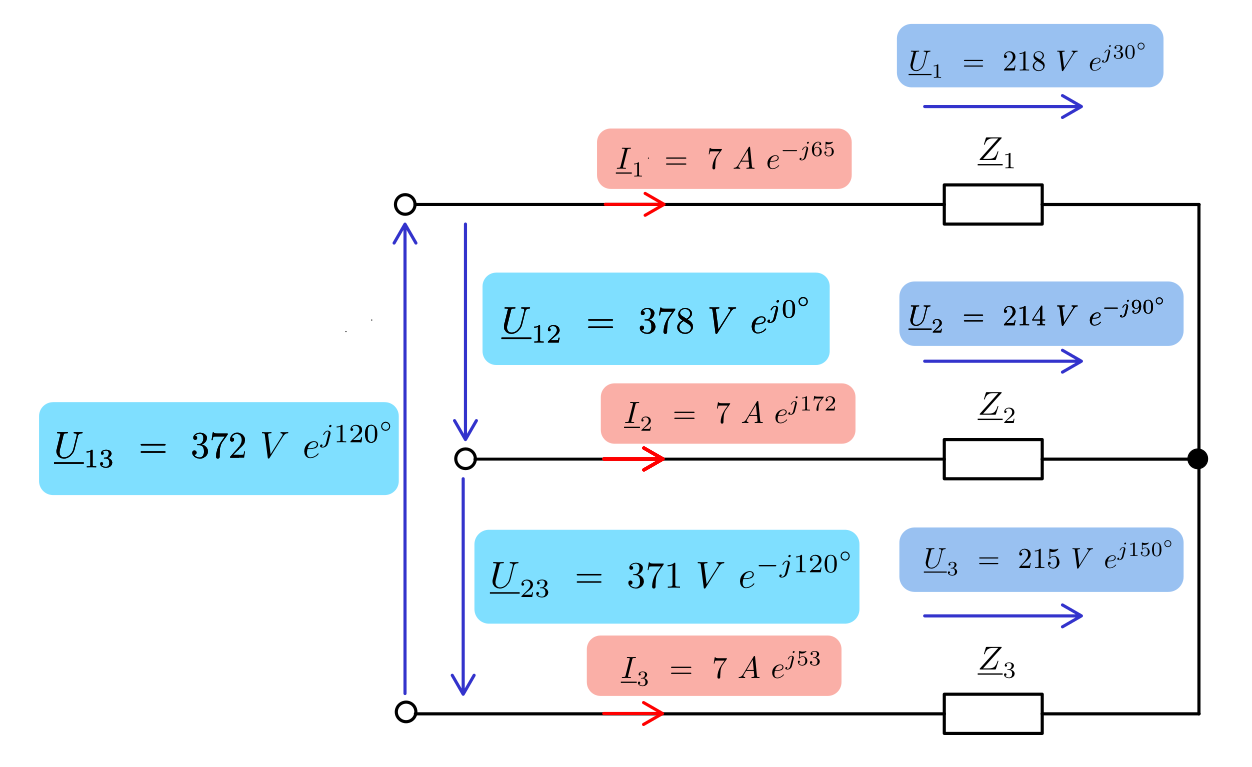
\includegraphics[width=0.75\textwidth]{img/4.2.1.1}
		      \end{center}
		      \caption{Zeigerdiagramm der Eingangsseite}\label{img:4.2.1.1}
	      \end{figure}

	      \begin{table}[h!]
		      \centering
		      \caption{Messwerte der Ausgangsseite Yy5 Symmetrischelast}
		      \begin{tabular}{lllll}
			      \\ \hline
			      Phasen     & $\underline{U}$ in $[V]$ & $\varphi_{U}$ in $[^\circ]$ & $\underline{I}$ in $[A]$ & $\varphi_{I}$ in $[^\circ]$ \\ \hline
			      $L1$       & $357$                    & $0$                         & $7,0$                    & $-46$                       \\
			      $L2$       & $347$                    & $120$                       & $7,0$                    & $-46$                       \\
			      $L3$       & $358$                    & $-120$                      & $6,7$                    & $-46$                       \\ \hline
			      Mittelwert & $354,000$                & $0,000$                     & $6,900$                  & $-46,000$                   \\ \hline\hline
		      \end{tabular}
	      \end{table}

	      \begin{table}[h!]
		      \centering
		      \caption{Brechnung der Ausgangsseite Yy5 Symmetrischelast}
		      \begin{tabular}{llllll}
			      \\ \hline
			      Phase      & $\varphi$ in $[^\circ]$ & $S$ in $[\SI{}{\kilo\volt\ampere}]$ & $P$ in $[\SI{}{\kilo\watt}]$ & $Q$ in $[\SI{}{\kilo\volt\ampere r}]$ & $\lambda$ in $[\ ]$ \\ \hline
			      $L1$       & $46$                    & $4,328$                             & $3,006$                      & $3,114$                               & $0,695$             \\
			      $L2$       & $46$                    & $4,207$                             & $2,923$                      & $3,026$                               & $0,695$             \\
			      $L3$       & $46$                    & $4,154$                             & $2,886$                      & $2,988$                               & $0,695$             \\ \hline
			      Mittelwert & $46$                    & $4,292$                             & $2,938$                      & $3,043$                               & $0,695$             \\ \hline\hline
		      \end{tabular}
	      \end{table}

	      \begin{figure}[h!]
		      \begin{center}
			      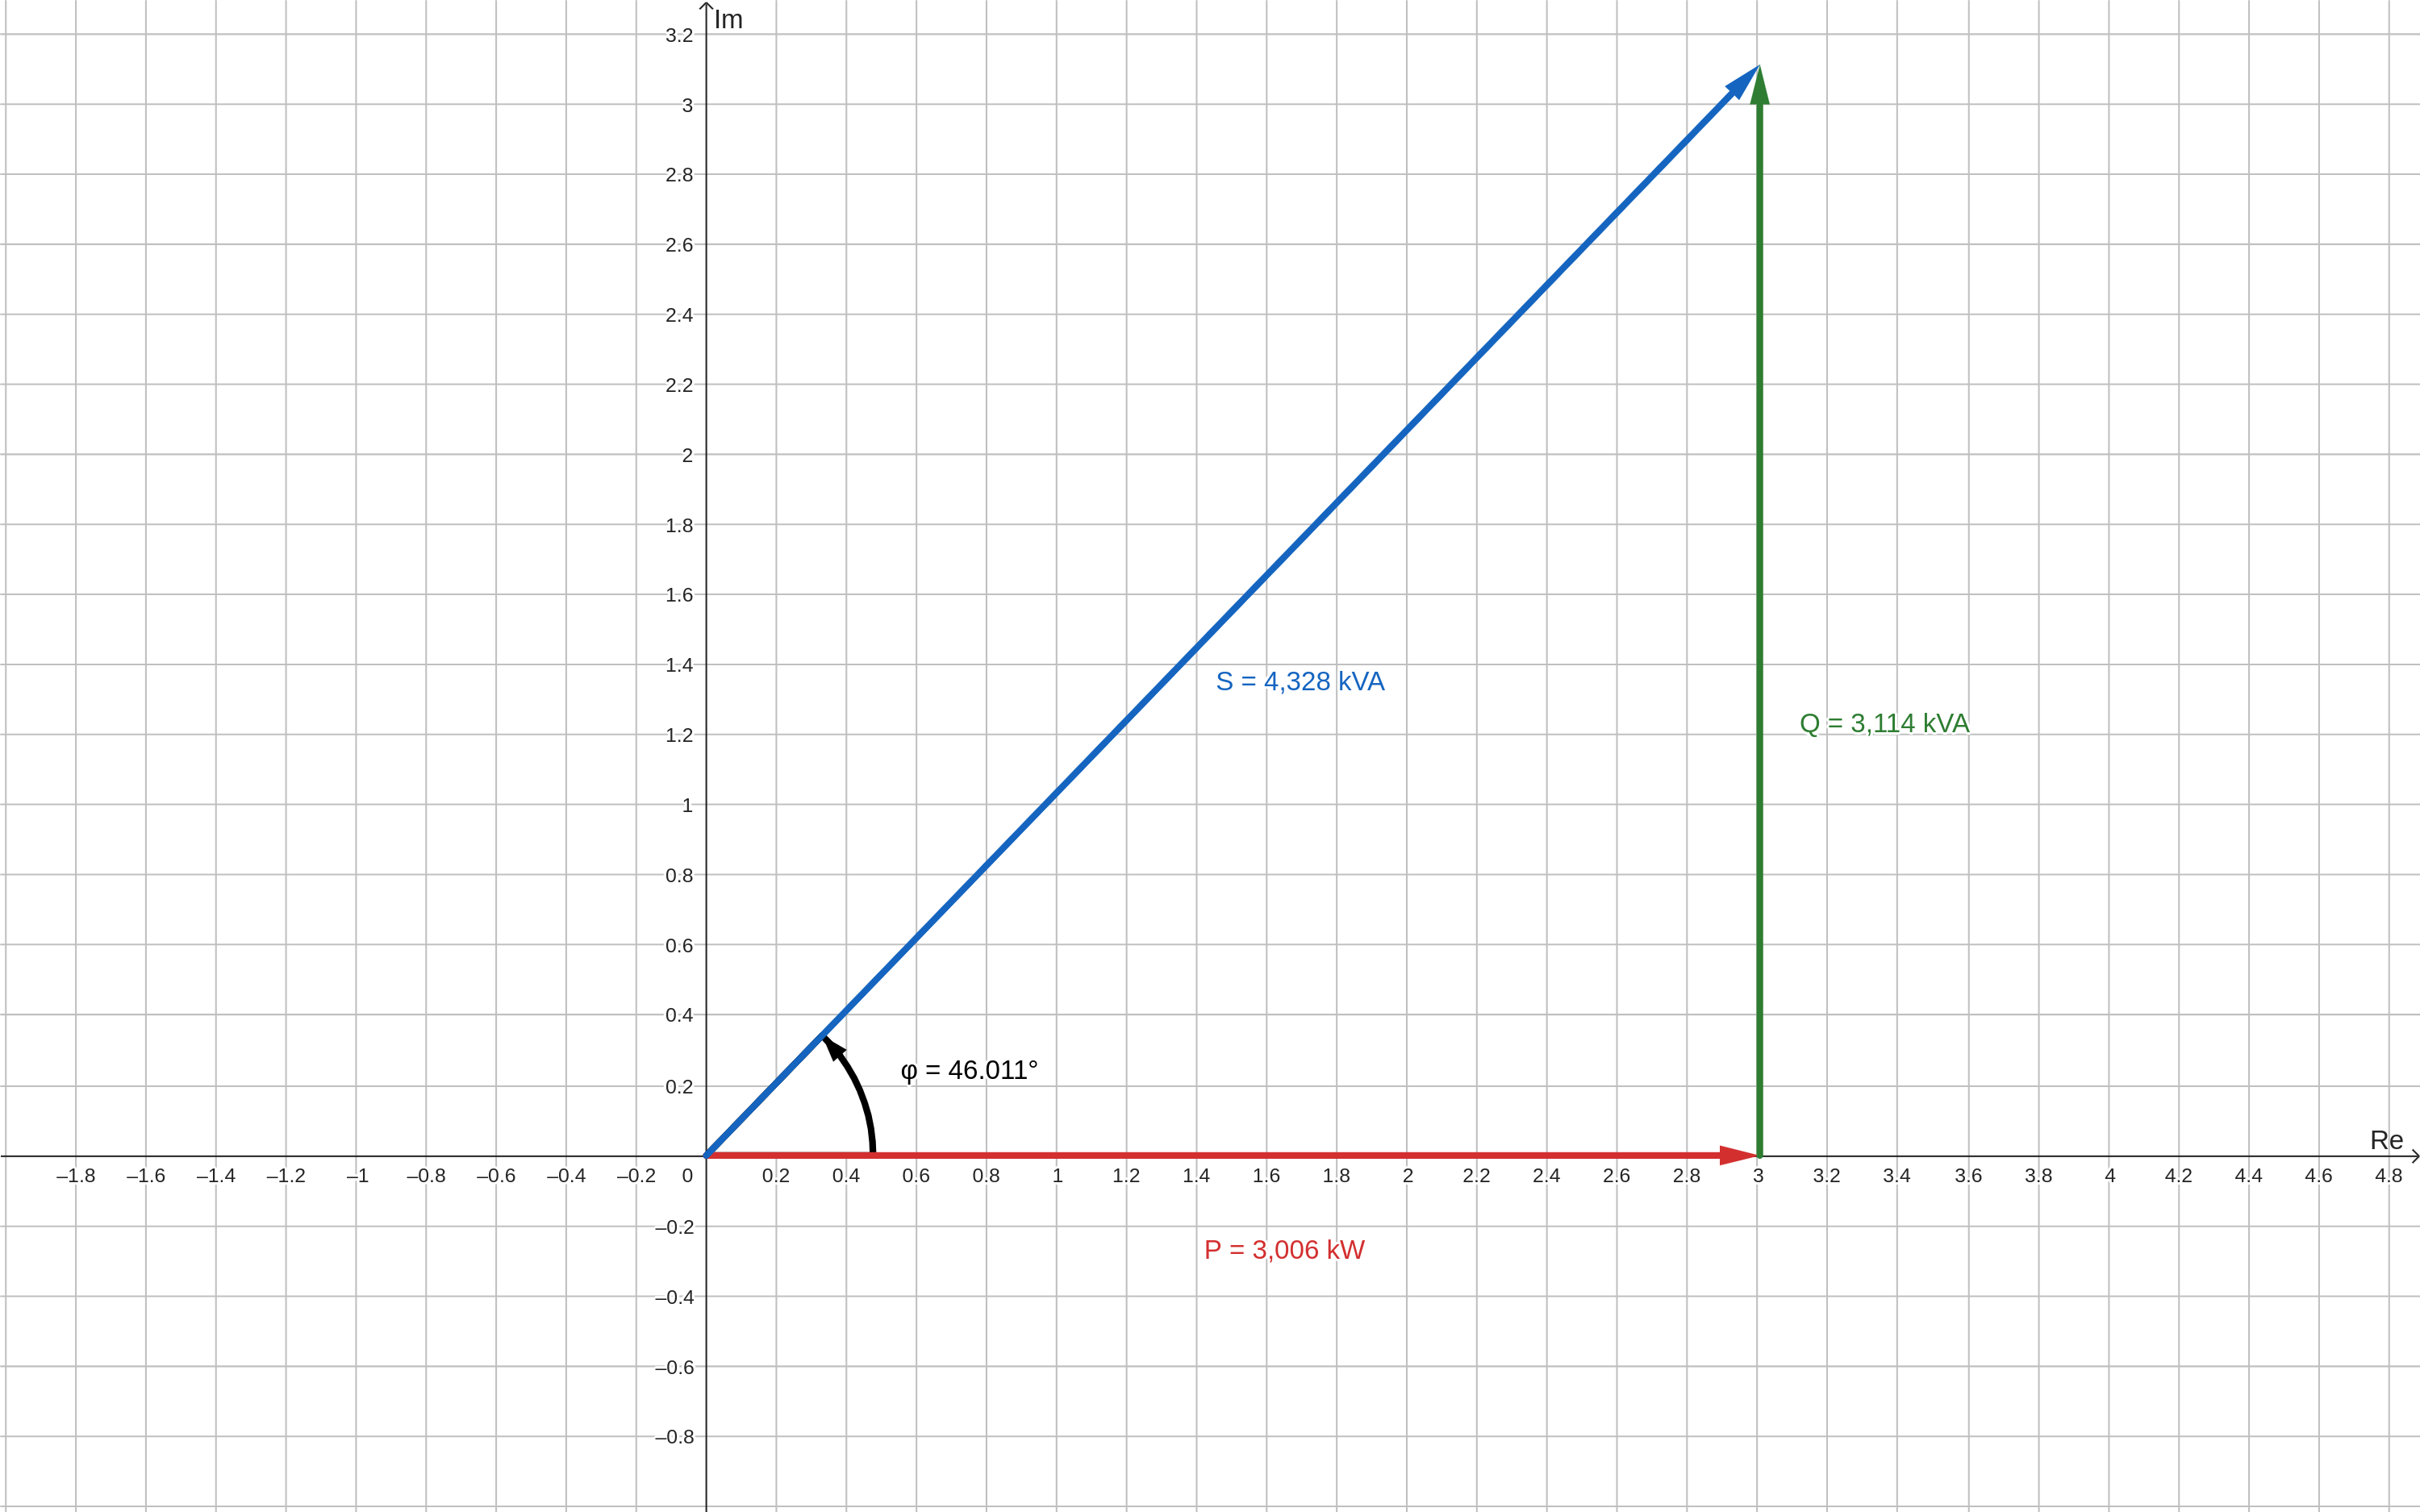
\includegraphics[width=0.75\textwidth]{img/4.2.1.2}
		      \end{center}
		      \caption{Zeigerdiagramm der Ausgangsseite}\label{img:4.2.1.2}
	      \end{figure}

	\item Berechnen Sie die Verlustleistung des Transformators sowie den Wirkungsgrad mit
	      den Ergebnissen aus 4.2(a).

	      \begin{align*}
		      S_{V} & = S_{e} - S_{a} \\
	      \end{align*}
	      \begin{figure}[!h]
		      \begin{center}
			      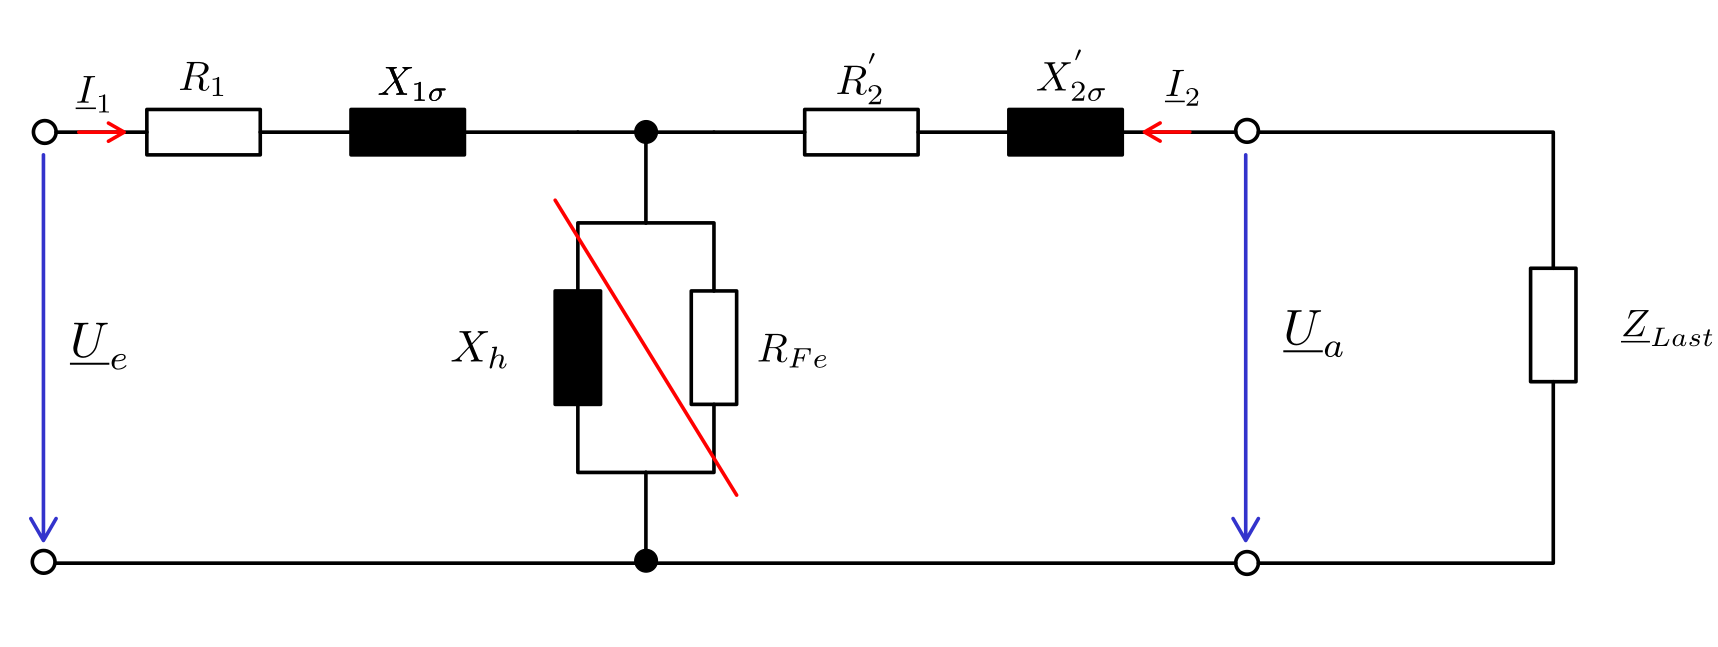
\includegraphics[width=0.75\textwidth]{img/4.2.2.1}
		      \end{center}
		      \caption{ESP für den Transformator im Lastbetrieb}\label{img:4.2.2.1}
	      \end{figure}

	\item Bestimmen Sie die Verlustleistung für 3.2(b) nach 2.1(d) und vergleichen Sie
	      das Ergebnis mit dem Wert aus 4.2(b). Begründen Sie Ihre Beobachtungen.
	      \newpage
	      \begin{minipage}[r]{0.5\linewidth}
		      \begin{align*}
			      P_{FE} & = P_0\ (\frac{U}{U_N})^2              \\
			      P_{FE} & = -43,1\ W\ (\frac{373\ V}{400\ V})^2 \\
			      P_{FE} & = -37,477\ W
			      \\
			      P_{Cu} & = P_K\ (\frac{I}{I_N})^2              \\
			      P_{Cu} & = 113\ W\ (\frac{7\ A}{7,2\ A})^2     \\
			      P_{Cu} & = 106,909\ W
		      \end{align*}
	      \end{minipage}
	      \begin{minipage}[l]{0.5\linewidth}
		      \begin{align*}
			      P_{V} & = P_{FE} \ +\ P_{Cu}                                  \\
			      P_{V} & = -37,477\ W + 106,909\ W                             \\
			      P_{V} & = 69,33\ W
			      \\
			      \eta  & = 1-\frac{P_{v}}{S}                                   \\
			      \eta  & = 1- \frac{69,33\ W}{\sqrt{3}\cdot 354\ V\cdot 7\ A } \\
			      \eta  & = 0,9838
		      \end{align*}
	      \end{minipage}

	\item Berechnen Sie aus den Messwerten nach 3.2(b) und dem Übersetzungsverhältnis ü
	      den relativen Spannungsfall $\Delta u'_2$!\\ \ \\

	      \begin{minipage}[r]{0.5\linewidth}
		      \begin{align*}
			      U_1 & = ü\cdot U_2            \\
			      ü   & = \frac{U_1}{U_2}       \\
			      ü   & = \frac{373\ V}{354\ V} \\
			      ü   & = 1,053                 \\
			      ü   & \approx 1
		      \end{align*}
	      \end{minipage}
	      \begin{minipage}[l]{0.5\linewidth}
		      \begin{align*}
			      I_2 & = ü\cdot I_1          \\
			      ü   & = \frac{I_2}{I_1}     \\
			      ü   & = \frac{6,9\ A}{7\ A} \\
			      ü   & = 0,985               \\
			      ü   & \approx 1
		      \end{align*}
	      \end{minipage}

	\item Bestimmen Sie anhand der Formeln (11) - (13) den relativen Spannungsabfall für
	      3.2(b).

	      \begin{align*}
		      \Delta u'_2 & = \frac{U_1\ -\ U'_2}{U_1}                       \\
		      \Delta u'_2 & = \frac{373\ V -\frac{373\ V}{\sqrt{3}}}{373\ V} \\
		      \Delta u'_2 & = 0,422                                          \\
	      \end{align*}
	      \begin{align*}
		      U_l         & = I_1(R_K\cos(\varphi_2)+X_K\sin(\varphi_2))                              \\
		      U_l         & = 7\ A\ (33,7\ \Omega\ \cos(-46^\circ)\ +\ 40,1\ \Omega\ \sin(-46^\circ)) \\
		      U_l         & = -38,728\ V                                                              \\
		      \\
		      U_q         & = I_1(R_K\cos(\varphi_2)+X_K\sin(\varphi_2))                              \\
		      U_q         & = 7\ A\ (33,7\ \Omega\ \sin(-46^\circ)\ +\ 40,1\ \Omega\ \cos(-46^\circ)) \\
		      U_q         & = 24,592\ V                                                               \\
		      \\
		      \Delta u'_2 & = 1+\frac{U_l}{U_1} - \sqrt{1-\frac{U_q}{U_1}}                            \\
		      \Delta u'_2 & = 1+\frac{-38,728\ V}{373,67\ V} - \sqrt{1-\frac{24,592\ V}{373,67\ V}}   \\
		      \Delta u'_2 & = 0,100\ 336
	      \end{align*}

	\item Vergleichen Sie die primär- und sekundärseitigen Spannungen und Ströme aus
	      3.2(b) und 3.2(c) miteinander.

\end{enumerate}
